\documentclass{article}
\usepackage{amssymb}
\usepackage{amsmath}
\usepackage{tikz}
\usepackage{pgfplots}

\usepackage{listings}
\usepackage{color}
\usepackage{enumitem}
\usepackage{pdfpages}
\usepackage{listings}
\usepackage{color}

\definecolor{codegreen}{rgb}{0,0.6,0}
\definecolor{codegray}{rgb}{0.5,0.5,0.5}
\definecolor{codepurple}{rgb}{0.58,0,0.82}
\definecolor{backcolour}{rgb}{0.95,0.95,0.92}

\lstdefinestyle{mystyle}{
    commentstyle=\color{codegreen},
    keywordstyle=\color{magenta},
    numberstyle=\tiny\color{codegray},
    stringstyle=\color{codepurple},
    basicstyle=\footnotesize,
    breakatwhitespace=false,
    breaklines=true,
    captionpos=b,
    keepspaces=true,
    numbers=left,
    numbersep=5pt,
    showspaces=false,
    showstringspaces=false,
    showtabs=false,
    tabsize=2
}

\lstset{style=mystyle}
\pgfplotsset{compat=1.15}
\newlist{alphalist}{enumerate}{1}
\setlist[alphalist,1]{label=\textbf{\Alph*.}}
\begin{document}
\section{R9.7}
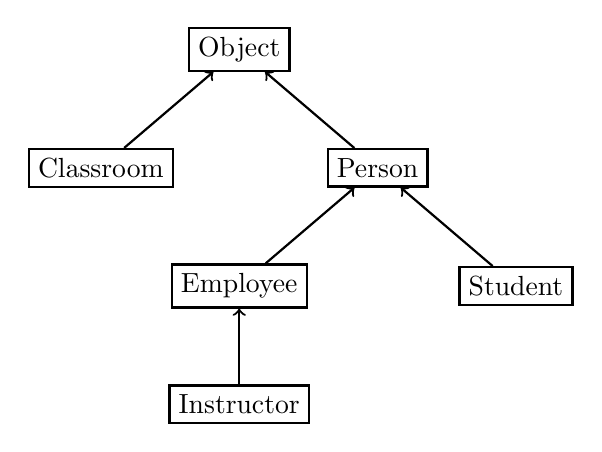
\begin{tikzpicture}[sibling distance=10em,
  every node/.style = {shape=rectangle,
    draw, align=center,
    top color=white, bottom color=white!20},
 ]
 \node {Object}[thick][<-]
 child { node {Classroom} }
 child { node {Person}
   child { node {Employee}
     child { node {Instructor} } }
   child { node {Student} } };
\end{tikzpicture}
\section{R9.11}
\begin{alphalist}
 \item Returns True
 \item Returns True
 \item Returns False
 \item Returns True
 \item Returns True
 \item Returns an error
\end{alphalist}
\section{R9.13}
Jj=(J)i\\
i can't be of type J.
\newpage
\section{R.11}
\subsection*{Student}
\begin{lstlisting}[language=Java]
class Student extends Person{
    private String Major = null;

    public Student(String name, int YOB, String major) {
        super(name, YOB);
        Major = major;
    }

    public void setMajor(String major) {
        Major = major;
    }

    public String getMajor() {
        return Major;
    }

    @Override
    public String toString() {
        return "Student{" +
                "Major: " + Major +","+
                "Name: " +getName()+", "+
                "Year: "+getYOB()+", "+
                '}';
    }
}

\end{lstlisting}
\subsection*{Student}
\begin{lstlisting}[language=Java]
class Student extends Person{
    private String Major = null;

    public Student(String name, int YOB, String major) {
        super(name, YOB);
        Major = major;
    }

    public void setMajor(String major) {
        Major = major;
    }

    public String getMajor() {
        return Major;
    }

    @Override
    public String toString() {
        return "Student{" +
                "Major: " + Major +","+
                "Name: " +getName()+", "+
                "Year: "+getYOB()+", "+
                '}';
    }
}

\end{lstlisting}
\subsection*{Person}
\begin{lstlisting}[language=Java]
public class Person {
    private String name;
    private int YOB;

    public String getName() {
        return name;
    }
    public int getYOB() {
        return YOB;
    }

    public void setName(String name) {
        this.name = name;
    }

    public void setYOB(int YOB) {
        this.YOB = YOB;
    }

    public Person(String name, int YOB) {
        this.name = name;
        this.YOB = YOB;
    }\end{lstlisting}
\end{document}
